%!TEX root = main.tex

% Introduction for negFE
\section{Introduction}
Information reconciliation and privacy amplification are the two
fundamental tasks for key derivation from noisy sources.  Roughly
speaking, information reconciliation takes two correlated
distributions $w$ and $w'$ and maps them to the same value while
minimizing what is leaked about that value.  Privacy amplification
converts the uncertainty in this mapped value to a uniform value
suitable for cryptography.  Applications areas include quantum key
agreement, biometrics, and physically uncloneable
functions~\cite{bennett1988privacy,dodis2008fuzzy}.

We focus on non-interactive versions of these problems~\cite{dodis2008fuzzy} as defined by secure sketches, which perform information-recon\-ciliation, and fuzzy extractors, which perform both information-recon\-ciliation and privacy amplification. A Secure Sketch consists of a pair of algorithms \emph{sketch} or $\sketch$ where:
\begin{enumerate}
\item $\sketch(w) = ss$ should reveal as little information as possible about $w$; and
\item $\sketch(w) =ss$ should allow one to reconstruct $w$ from a nearby $w'$. That is, it should be the case that for all nearby $w', \rec(w', ss) = w$.  In the above, ``nearby'' is $w'$ such that $\dis(w,w')\le t$ for  distance metric $\dis$ and distance $t$.
\end{enumerate}
These two properties are in tension because allowing recovery of $w$ requires information about $w$.  The most natural (inefficient) construction is for $ss$ to be a pairwise independent~\cite{carter1977universal} hash $h$ of $w$~\cite{skoric2009efficient,fuller2016fuzzy,woodage2017new,fuller2020fuzzy}. The hash $h$ should be long enough so that $\{w | h(w) = y \wedge w' s.t.\,\dis(w, w')\le t\} =1$ and short enough so $\{w| h(w) = y\}$ is large. Constructions are also known based on error-correcting codes.  In fact, upper bounds on the unpredictability of $w | ss$ are related to the size of the best error-correcting codes~\cite{dodis2008fuzzy,fuller2020computational}. 

Given a good information reconciliation, one can achieve privacy amplification using an average-case randomness extractor~\cite{nisan1993randomness} to convert $w$ into a uniform value.
  Fuzzy extractors perform both information reconciliation and privacy amplification.  They consist of a pair $(\gen, \rep$).  Intuitively, $\gen$ converts a value $w$ into a uniform value and $\rep$ reproduces that value for any nearby $w'$.  Notationally, $(r, p)\leftarrow \gen(w)$ should be indistinguishable from $(u, p)$ where $u$ is a truly random value.  On the correctness side, it should be the case that for all $w'$ such that $\dis(w, w')\le t$ then $\rep(w', p) =r$.  
  Both $\sketch$ and $\gen$ are allowed to have private internal randomness.  
  
  
Since noisy sources come from the physical world, an important goal
  is to be able to support as many distributions $W$ as possible. This goal is the focus of this work. 
  Throughout the Introduction, we use the notation of fuzzy extractors
  and note when there are material differences for secure sketches.
  Fuller, Reyzin, and Smith~\cite{fuller2016fuzzy,fuller2020fuzzy}
  identified the notion of fuzzy min-entropy $\Hfuzz(W)$ which
  measures the adversary's success when given oracle access to
  $\rep(\cdot, p)$ but is unable to learn anything from the value $p$.
  Mathematically, fuzzy min-entropy quantifies the weight of the heaviest ball
  in the probability mass function of $W$.  That is,
\[
\Hfuzz(W):= -\log{\max_{w'} \sum_{w | \dis(w, w')\le t} \Pr[W=w]}.
\]A primary goal of fuzzy extractor research is to build a single fuzzy extractor that works for the family of all distributions $\Wallfuzz = \{ W | \Hfuzz(W) = \omega(\log \lambda)\}$ for some security parameter $\lambda$.  We call such a fuzzy extractor \emph{universal} as it simultaneously works for any secureable distribution $W$. 
If one desires computational security, a universal fuzzy extractor is achievable using general obfuscation~\cite{BarakBCKPS13,BitanskyCKP14,bitansky2017virtual} or under specific number-theoretic assumptions~\cite{galbraith2019obfuscated}. 


The situation for information-theoretic security is more
complicated.\footnote{Fuzzy extractors were first designed as an
  information-theoretic primitive because of strong connections to
  randomness extraction and coding theory.  Many computational
  constructions use an information-theoretic secure
  sketch~\cite{wen2018robustly,wen2019generic}.  (Exceptions exist
  such as the universal constructions listed above and constructions
  for distributions with additional
  properties~\cite{apon2017efficient,alamelou2018pseudoentropic,fuller2020computational,canetti2021reusable}.)
}  Fuller, Reyzin, and Smith~\cite{fuller2020fuzzy} showed that it is
impossible to build a universal fuzzy extractor with
information-theoretic security.  More precisely, they constructed a
family of distributions $\mathcal{W}' = \{ W_z \}$ and showed that any
fuzzy extractor $(\gen, \rep)$ must be insecure for an average member
of $\mathcal{W}'$. We let $Z$ describe a uniformly chosen index for
the family $\mathcal{W'}$, and use the notation $W_Z$ to indicate the
distribution arising from this choice of $Z$. Importantly, in the
impossibility result the adversary knows the entire description of the
chosen distribution (that is, $W_Z$) but not the
individual point $w$ that was input to $\gen$.

On the positive side, multiple works~\cite{hayashi2014secret,hayashi2016secret,fuller2016fuzzy,woodage2017new,tyagi2017universal,TVW18,LA18,fuller2019continuous,fuller2020fuzzy} presented a construction that works for each $W_Z\in \Wallfuzz$.  This is called the \emph{distribution-sensitive} setting as $\gen$ also knows the entire probability mass function $Z$ of the chosen $W_Z$, denoted as $\gen_{W_Z}, \rec_{W_Z}$.  All constructions in this line are computationally inefficient; for an input point $w$ they look up the probability that $\Pr[W_Z=w]$ and the probability of points $w'$ where $\dis(w, w')\le t$.  
%Thus, there is a large gap between the state of affairs with computational and information-theoretic security.  With computational security, universal fuzzy extractors are possible.  With information-theoretic security universal fuzzy extractors are impossible.  Furthermore, known distribution-sensitive fuzzy extractors require information about $W$ proportional to its description.  

We show this inefficiency is unavoidable:
\begin{displayquote}
\textbf{Any distribution-sensitive information-theoretic fuzzy extractor requires an exponential amount of information about the distribution $W$.} 
\end{displayquote} 
Our results are for the Hamming metric over $\zo^n$. Below we present the two informal theorems for fuzzy extractors (see Theorem~\ref{thm:main theorem}) and secure sketches (see Theorem~\ref{thm:main theorem ss}) respectively.  For a value $p\in [0,1]$ let $h_2$ be the binary entropy of $p$. 

\begin{theorem}[Informal Theorem~\ref{thm:main theorem}]
Consider $\zo^n$ and $t< n/2$ be a distance parameter.  Let $\mathcal{W}_\gamma=\{W | \Hfuzz(W) = \gamma\}$.  Let $c>0$ be a constant and suppose that \[
\gamma \le n\cdot\min\left\{(1-h_2(t/n)) +o(1), \frac{1-\Theta(c)-h_2(1/2-t/n)}{3}\right\}.
\]
 For a quarter of $W \in \mathcal{W}_\gamma$ there is no fuzzy extractor that simultaneously has 1) no error 2) is of size at most $2^{\gamma+cn}$ 3) extracts keys of length $\omega(\log n)$ that are within statistical distance $1/3-\ngl(n)$ to a uniform key.
\end{theorem}

For the setting of secure sketches, we allow the secure sketch to have some bounded probability $\delta$ that the output of $\rec(ss, w') \neq w$.  We state the informal theorem below.  
\begin{theorem}[Informal Theorem~\ref{thm:main theorem ss}]
Consider $\zo^n$ and $t< n/2$ be a distance parameter.  Let $\mathcal{W}_\gamma=\{W | \Hfuzz(W) = \gamma\}$.  Let $\delta<1/4$ be the error of the secure sketch, let $c>0$ be a constant and suppose that \[
\gamma \le n\cdot\min\left\{(1-h_2(t/n)) +o(1), c_\delta h_2(t/n)-\Theta(c)-\Theta(1/n)\right\}.
\]
where $1/3\le  c_\delta \le 2/3$ and depends on $h_2(\delta)$. 
 For $2^{-4}$ fraction of $W \in \mathcal{W}_\gamma$ there is no secure sketch of
size of at most $2^{\gamma+cn}$ that
 retains unpredictability of $w|ss$ of at  least $4$.
\end{theorem}

\begin{figure}[t]
\centering
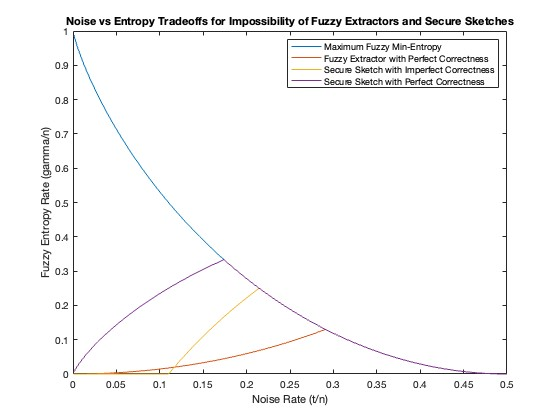
\includegraphics[width=.9\textwidth]{EntropyvsError.jpg}
\caption{The region of error rate $t/n$ ($x$-axis) and fuzzy entropy rate $\gamma/n$ (y-axis) pairs for which the two negative results apply.  The six curves are maximum fuzzy min-entropy $\gamma/n = (1-h_2(t/n))$, Theorem~\ref{thm:main theorem}, Theorem~\ref{thm:main theorem ss} with $\delta=.25$,  Theorem~\ref{thm:main theorem ss} with $\delta =0$, \cite[Theorem 5.1]{fuller2020fuzzy} and \cite[Theorem 7.2]{fuller2020fuzzy}. The parameter $\delta$ is how frequently the secure sketch is allowed to be incorrect.  We consider fuzzy extractors with perfect correctness where $\delta=0$.}
\label{fig:param regime}
\end{figure}
 The relevant parameter regimes of impossibility are shown in Figure~\ref{fig:param regime}.  The two most important parameters are the noise rate $t/n$ and the fuzzy entropy rate $\gamma/n$. The area under the curves represents parameters where the construction is impossible for the fraction of distributions in the informal theorems unless one has algorithms of $2^{\Theta(n)}$ size.
In spirit, our result rules out constructions that do not have a full description of the probability mass function written in their description.  Our results are actually stronger, restricting only the amount of information about $W$ not the running time or size.  


%There are (at least) two natural interpretations of the above result: 1) that fuzzy min-entropy does not measure the suitability of distributions for key derivation or 2) that efficient fuzzy extractors are an inherently computational object.
%
%\paragraph{The notion of fuzzy min-entropy}
%One of the principal components of a fuzzy extractor is privacy amplification where smooth conditional min-entropy~\cite{renner2005simple} is a necessary and sufficient condition.  This rather precisely characterizes the regime
%of feasibility for efficient privacy amplification as an
%information-theoretic task.  However, the gap between necessary and sufficient conditions for \emph{efficient} primitives that perform information reconciliation appears much wider. The only known efficient constructions for information reconciliation fall into one of two categories:
%\begin{description}
%\item[High entropy] If the source $W$ has high entropy $\Hoo(W)\ge \omega(\log n) + \log{|B_t|}|$ (where $|B_t|$ is the size of a Hamming ball of radius $t$) then one can build a good secure sketch by writing down the syndrome of an error correcting code which corrects $t$ errors.  This syndrome construction  leaks at least $\log{|B_t|}$ bits of information about $W$.\footnote{A construction that leaks only $\log{|B_t|}$ bits about $W$ requires a perfect code which are rarely achievable.}  Unfortunately, this construction provides no guarantee when $\Hoo(W)< \log{|B_t|}$ which is the case for biometrics, see \cite[Proposition 1]{canetti2021reusable} and \cite[Introduction]{simhadri2019cryptographic}.
%\item[Highly structured] Sources where each bit is i.i.d.\ can be analyzed using Shannon entropy.  In this setting, key rate asymptotically approaches $\Hfuzz(W)$ if one assumes the second reading $w'$ will be uniformly distributed in the ball around the first reading~\cite[Theorem 2]{tuyls2004capacity}.  Unfortunately, coordinates of real-physical sources are rarely i.i.d.~\cite{daugman2004}.
%\end{description}
%
%Unfortunately, there isn't an obvious sufficient condition to adopt
%rather than fuzzy min-entropy.  Various weaker structured conditions
%have been used in the computational regime but with little evidence
%that physical sources have these properties~\cite[Figure
%1]{demarest2021code} and \cite{simhadri2019cryptographic}. Thus, a desirable
%research goal is to identify statistical properties possessed by physical
%sources that bypass our negative results.

As we discuss below, our results are relatively straightforward using only first and second-moment bounds.  We do not view the proofs as the contribution of this work.  \textbf{Our theorems are crucial for the future of information-theoretic fuzzy extractors: one must use properties of a noisy source beyond fuzzy min-entropy to provide an efficient construction.}  Most deployed constructions of fuzzy extractors use an information-theoretic information-reconciliation component and are thus subject to our results. 


%\paragraph{Fuzzy extractors are computational objects} The other
%natural explanation of the result is that non-interactive information
%reconciliation should be considered a computational object. This is
%our preferred interpretation since one can build universal (and
%efficient) fuzzy extractors if computational security suffices.  We
%note that the only known constructions assume either general
%obfuscation~\cite{BarakBCKPS13,BitanskyCKP14,bitansky2017virtual} or
%specific number-theoretic assumptions that are not well
%studied~\cite{galbraith2019obfuscated}. Thus, an important direction
%of research is to understand the required assumptions to build
%efficient, universal fuzzy extractors with computational security.


\subsection{Proof Techniques}
Our results are information-theoretic. As discussed above, we shall
consider a family of distributions $\mathcal{W} = \{ W_z \}$, let $Z$
denote a uniformly random index for $\mathcal{W}$, and let $W_Z$
denote the distribution determined by this choice of $Z$.
% \anote{I am confused by this, is $W_Z$ a distribution or a random variable? It looks from the next sentence as though it is a distribution, in which case the language should be changed.}
Lastly, we use $w\leftarrow W_Z$ to
denote sampling a point from the distribution.  We show the
impossibility of two types of fuzzy extractors:
\begin{description}
\item[Def.~\ref{def:fe distributional}] (Universal) Fuzzy extractors with distributional advice.  This is triple of algorithms $(\advice, \gen, \rep)$ designed to work for all $W_Z \in \mathcal{W}$ where $\mathcal{W}$ consists of all distributions with a certain amount of fuzzy min-entropy for a fixed error tolerance $t$.  However, the fuzzy extractor is given information about $Z$.  Namely, there is a deterministic algorithm $\advice = \advice(Z)$. Then both $\gen$ and $\rep$ are given $\advice$. Define $w\leftarrow W_Z$ and $(r, p) \leftarrow \gen(w, \advice)$, it should be true that 
\[
(r, p, Z) \approx (U, p, Z).
\]
Note that all information about $Z$ given to $\gen$ is contained in $\advice$ and the point $w$.
\item[Def.~\ref{def:fe}] Fuzzy extractors for a specific distribution $W$ that are required to have a bounded size description of $(\gen, \rep)$.
\end{description}

We show impossibility of building a fuzzy extractor with distributional advice of length $\ell$ for $\mathcal{W}$ implies impossibility of building a space bounded fuzzy extractor for length $\ell$ (Lemma~\ref{lem:distributional advise suffices}). 
The core of our negative results is to show the impossibility of building fuzzy extractors with distributional advice.   

We perform a brief overview of Fuller, Reyzin, and Smith's~\cite{fuller2020fuzzy} impossibility result.
%\paragraph{Review of Fuller, Reyzin, and Smith~\cite{fuller2020fuzzy}}
The correctness constraint of a fuzzy extractor says that for $(r, p)\leftarrow \gen(w)$ for all $w'$ close to $w$ the correct key is reproduced, i.e., $\rep(w', p)=r$.  As such, one can partition the input space $\zo^n$ by what value of $r$ the point  $v\in \zo^n$ produces.  Values $v$ that could have produced  $r$ will be at least distance $t$ from the boundary of this partition, we call the set of such $v$, $\viable_{r,p}$.  $\viable_{r,p}$ can be bounded geometrically using the isoperimetric inequality~\cite{harper1966optimal}.  This bound applies for any distribution over the inputs $w$.

Consider the following simple distinguisher for a triple $r, p, z$.  One computes the key partition described above and the set $\viable_{r,p}$. If $\viable_{r,p} \cap W_z $ is empty output the key is random, otherwise output key is real. 
The core of Fuller, Reyzin, and Smith's impossibility was to build a family $\mathcal{W}^{FRS}$ with three properties:
\begin{enumerate}
\item The distribution was $2$-universal~\cite{carter1977universal}, so the remainder of the distribution was unknown conditioned on the input $w$. 
\item Distributions $W_Z \in \mathcal{W}^{FRS}$ shared few points, and 
\item Each distribution $\mathcal{W}^{FRS}$ had fuzzy min-entropy.
\end{enumerate}
Together these three properties meant that for any partition most distributions $W_Z$ would have few nonempty interiors and the real key could be distinguished from a uniform key.  
The family is as follows: let $\mathbf{C}$ be a linear error-correcting code with distance $t$, let $\mathbf{H}$ be its syndrome, let $c$ be a coset.  Then each $Z = (\mathbf{H}, c)$ is the set of all points $\{w \mid \mathbf{H} w = c\}$.

\paragraph{Moving to the distributional advice setting}
To set notation for the distributional advice game, we consider the following game for a tuple of algorithms $(\advice, \gen, \rep)$:
\begin{enumerate}
\itemsep0em
\item A uniform sample from $W_Z \leftarrow \mathcal{W}$ where $Z$ describes the distribution. 
\item A bounded length $\advice = \advice(Z)$ is computed.
\item One computes $w\leftarrow W_Z$.
\item The algorithm computes $(r, p)\leftarrow \gen(w, \advice)$.
\item The adversary is given either $(r, p, Z)$ or $(u, p, Z)$ for a uniform $u$. 
\end{enumerate}

In \cite{fuller2020fuzzy}, the only information that $\gen$ had about $Z$ was the input point $w$.  In our setting, $\gen$ gets $\advice$.  Fuller, Reyzin, and Smith's family had a short description so $\advice$ could completely write $Z$, allowing $\gen$ to align the interior of the parts with points in $W_Z$.  Thus, extending the result requires a long description that can't be compressed.  The natural candidate is the set of all distributions $W_Z\in\mathcal{W}$ with fuzzy min-entropy at least $\gamma$. 

We show there are few distributions with $2^k$ points chosen uniformly without replacement that do not have fuzzy min-entropy $\gamma$ where $k = \gamma +cn$ for some $c>0$.  We call this set of distributions $U_{n,k}$ and use this set of distributions throughout most of our proofs. Let $w_1,...., w_{2^k}$ be the points with nonzero probability.  As long as $|\advice|$ is shorter than $2^k$, most points $w_i | \advice$ are unpredictable.  %This argument must account for the fact that $\advice$ can choose to completely determine some points or provide equal information about all points. 

The techniques for the secure sketch setting are similar, however, there are stronger geometric bounds on the number of viable points because secure sketches imply Shannon error correcting codes~\cite{dodis2008fuzzy,fuller2020computational}.  Our result considers a secure sketch that retains smooth min-entropy instead of min-entropy.  This is so we can use $U_{n,k}$ throughout the proof and show this implies the hardness of building a secure sketch for all distributions with sufficient fuzzy min-entropy.  Our final result also applies to secure sketches that retain non-smooth conditional min-entropy.

Importantly, both results operate generically in the size of the maximum number of viable points for the relevant primitive.  Such bounds have been well established in the literature due to their connections with coding theory.  This means if one can provide a new bound on fuzzy extractor or secure sketch quality this can be directly used in our results. 


\paragraph{Discussion}
As noted above, our proofs are relatively simple but have strong implications for the future of fuzzy extractors, new designs or analyses are necessary.

Our fuzzy extractor result requires the $|r| = \omega(\log n)$.  This is in contrast to Fuller, Reyzin, and Smith~\cite{fuller2020computational} who showed an impossibility for a key length of $3$.\footnote{Our result for secure sketches requires them to retain at least $4$ bits of min-entropy about the input in comparison with \cite{fuller2020computational} which required the sketch to maintain $3$ bits of entropy.} This change comes because $\advice$ can supply a lot of information about a small number of points in $W_Z$, allowing $\gen$ to ensure that some $\viable_{r,p}$ are nonempty. Furthermore, all bounds are weaker than those of Fuller, Reyzin, and Smith.  The core of the difference is that since $\mathcal{W}^{FRS}$ the adversary received entirely new information by the leftover hash lemma~\cite{haastad1993construction,barak2011leftover}. In our setting, we argue about the expected number of points in $W_Z$ that are included in the $\viable$ region. 

Our secure sketch result also considers an object that retains smooth conditional min-entropy~\cite{renner2005simple}.  %Smooth conditional min-entropy means that one is statistically close to a distribution with min-entropy.  Setting the closeness parameter to $0$ gives traditional conditional min-entropy.  This is so we can conduct the argument using $U_{n,k}$ and ``smooth'' to the family where all distributions have fuzzy min-entropy. 
Smooth conditional min-entropy is the necessary and sufficient condition for privacy amplification using a randomness extractor. 


\paragraph{Organization} The rest of this work is organized as follows, Section~\ref{sec:prelim} covers preliminaries including the relevant definitions of fuzzy extractors and secure sketches.  Section~\ref{sec:fe} presents the negative result for fuzzy extractors including a proof outline, and Section~\ref{sec:ss} presents the negative result for secure sketches.


%%% Local Variables:
%%% mode: latex
%%% TeX-master: "main"
%%% End:
